\section{Results}
\label{sec:results}

\subsection{Cohort Characteristics, Data Audit, and Split-Geometry Findings}
Of 368,132 isolated-CABG procedures across 1,091 U.S.\ centers, skip-logic resolution yielded \textbf{367,695 labeled procedures} (437 excluded) with \textbf{89,337 treatment-requiring POAF events (24.30\%)}. Baseline clinical, procedural, and outcome profiles were tightly balanced between full development (1,017 hospitals, $N=346{,}454$, POAF 24.30\%) and strictly unseen external validation (74 centers, $N=21{,}241$, 5,160 events, POAF 24.29\%, 0.0\% overlap; Table~\ref{tab:cohort_baseline}), with $|\mathrm{SMD}| < 0.10$ across every baseline feature and all nine U.S.\ Census divisions matching within 0.18~pp.

\begin{table*}[t]
\centering
\tablefont
\caption{\ct{Baseline Patient, Clinical, Procedural, and Outcome Characteristics Across the National STS ACSD v2.81 Cohorts (1,091 U.S.\ Surgical Centers, 2014--2017).}}
\label{tab:cohort_baseline}
\setlength{\tabcolsep}{5.0pt}
\renewcommand{\arraystretch}{1.04}
\begin{tabularx}{\textwidth}{@{}Yrrrr@{}}
\toprule
\thd{Characteristic} & \thd{Full Development} & \thd{Nested 50k Benchmark} & \thd{Unseen External Test} & \thd{SMD$^{\dagger}$} \\
 & \thd{($N=346{,}454$; 1,017 ctr)} & \thd{($N=50{,}000$; 1,017 ctr)} & \thd{($N=21{,}241$; 74 ctr)} & \thd{(Dev vs.\ Test)} \\
\midrule
\multicolumn{5}{@{}l}{\textit{Demographics and Anthropometry}} \\
\quad Age, mean $\pm$ SD, yr & 65.1 $\pm$ 10.1 & 66.4 $\pm$ 10.0 & 65.2 $\pm$ 10.1 & 0.009 \\
\quad Female sex & 87,423 (25.2\%) & 12,093 (24.2\%) & 5,172 (24.4\%) & 0.020 \\
\quad White race & 285,838 (82.5\%) & 41,977 (84.0\%) & 17,206 (81.0\%) & 0.039 \\
\quad Black race & 26,750 (7.7\%) & 3,413 (6.8\%) & 1,822 (8.6\%) & 0.031 \\
\quad Asian race & 11,889 (3.4\%) & 1,648 (3.3\%) & 842 (4.0\%) & 0.028 \\
\quad Hispanic or Latino ethnicity & 26,921 (7.8\%) & 3,583 (7.2\%) & 1,433 (6.8\%) & 0.039 \\
\quad Body-mass index, mean $\pm$ SD, kg/m$^2$ & 30.1 $\pm$ 6.0 & 30.1 $\pm$ 6.0 & 30.0 $\pm$ 6.0 & 0.014 \\
\quad Body surface area, mean $\pm$ SD, m$^2$ & 2.01 $\pm$ 0.24 & 2.02 $\pm$ 0.24 & 2.01 $\pm$ 0.24 & 0.008 \\
\addlinespace[3pt]
\multicolumn{5}{@{}l}{\textit{Preoperative Clinical Comorbidities and Cardiac Substrate}} \\
\quad Hypertension & 306,810 (88.6\%) & 44,569 (89.1\%) & 19,032 (89.6\%) & 0.033 \\
\quad Diabetes mellitus & 168,522 (48.6\%) & 24,025 (48.0\%) & 10,456 (49.2\%) & 0.012 \\
\quad Heart failure (current or prior) & 75,070 (21.7\%) & 11,333 (22.7\%) & 5,018 (23.6\%) & 0.047 \\
\quad NYHA class III or IV & 35,307 (10.2\%) & 5,449 (10.9\%) & 2,511 (11.8\%) & 0.052 \\
\quad Prior myocardial infarction & 180,339 (52.0\%) & 26,134 (52.3\%) & 10,960 (51.6\%) & 0.009 \\
\quad Chronic lung disease & 82,357 (23.8\%) & 12,200 (24.4\%) & 4,643 (21.9\%) & 0.045 \\
\quad Peripheral vascular disease & 46,703 (13.5\%) & 7,052 (14.1\%) & 2,688 (12.7\%) & 0.025 \\
\quad Cerebrovascular disease & 68,057 (19.6\%) & 10,323 (20.6\%) & 3,959 (18.6\%) & 0.025 \\
\quad Chronic kidney disease (eGFR $<60$) & 72,267 (20.9\%) & 11,068 (22.1\%) & 4,561 (21.5\%) & 0.015 \\
\quad Preoperative dialysis & 9,939 (2.9\%) & 1,435 (2.9\%) & 612 (2.9\%) & 0.001 \\
\quad Recorded preoperative AF history & 1,762 (0.5\%) & 282 (0.6\%) & 138 (0.7\%) & 0.018 \\
\quad Left ventricular EF, mean $\pm$ SD, \% & 52.4 $\pm$ 12.2 & 52.3 $\pm$ 12.3 & 52.4 $\pm$ 12.1 & 0.001 \\
\quad Serum creatinine, mean $\pm$ SD, mg/dL & 1.18 $\pm$ 1.06 & 1.19 $\pm$ 1.06 & 1.20 $\pm$ 1.10 & 0.018 \\
\quad CKD-EPI 2021 eGFR, mL/min/1.73\,m$^2$ & 77.7 $\pm$ 23.5 & 76.5 $\pm$ 23.4 & 77.1 $\pm$ 23.6 & 0.025 \\
\addlinespace[3pt]
\multicolumn{5}{@{}l}{\textit{Surgical Acuity, Anatomy, and Preoperative Medications}} \\
\quad Three-vessel coronary disease & 264,116 (76.2\%) & 38,363 (76.7\%) & 16,465 (77.5\%) & 0.031 \\
\quad Elective operative status & 129,234 (37.3\%) & 18,690 (37.4\%) & 7,887 (37.1\%) & 0.004 \\
\quad Urgent operative status & 202,366 (58.4\%) & 29,130 (58.3\%) & 12,439 (58.6\%) & 0.003 \\
\quad Emergent or salvage status & 14,810 (4.3\%) & 2,173 (4.3\%) & 910 (4.3\%) & 0.001 \\
\quad Preoperative $\beta$-blocker therapy & 312,486 (90.2\%) & 45,027 (90.0\%) & 18,507 (87.1\%) & 0.097 \\
\quad Preoperative amiodarone therapy & 21,722 (6.3\%) & 2,935 (5.9\%) & 1,120 (5.3\%) & 0.043 \\
\addlinespace[3pt]
\multicolumn{5}{@{}l}{\textit{Primary Outcome (Treatment-Requiring New-Onset POAF)}} \\
\quad \textbf{POAF events (STS \texttt{COtAFib})} & \textbf{84,177 (24.30\%)} & \textbf{25,000 (50.0\%)} & \textbf{5,160 (24.29\%)} & \textbf{0.0002} \\
\bottomrule
\end{tabularx}
\par\smallskip\raggedright\fontsize{7.5}{9.4}\selectfont\color{sub}
$^{\dagger}$Standardized mean difference (SMD) comparing the natural-prior full development cohort (1,017 hospitals) with the strictly hospital-disjoint unseen external validation cohort (74 hospitals; 0.0\% hospital overlap). Every clinical characteristic exhibits $|\mathrm{SMD}| < 0.10$, and all nine U.S.\ Census divisions match within 0.18 percentage points. The nested 50,000-patient benchmark is class-balanced (25,000 POAF / 25,000 controls) strictly within the same 1,017 development hospitals and recalibrated back to natural clinical prevalence using the development-only Bayes offset ($-1.1365$).
\end{table*}


Center-level POAF incidence varied nearly threefold across 928 centers with $\ge 100$ cases, spanning 12.2\% to 34.2\% (5th--95th percentile; median 24.1\%, SD~6.68~pp; Figure~\ref{fig:study_design}B). Default calendar-2017 splitting ($N=61{,}552$, 99.5\% hospital overlap) masked severe transport error: an identical 207-feature CatBoost model scored 0.6778 on default 2017 cases yet dropped $-1.99$ AUC points to \textbf{0.6579} on 2017 operations at strictly unseen hospitals ($n=3{,}555$, 63 centers; Figure~\ref{fig:study_design}C). Multivariate anticlustering eliminated overlap while cutting worst-case covariate imbalance 3.5-fold ($\mathrm{Max}\,|\mathrm{SMD}|$: $0.3572 \to 0.1028$) and 32-D Energy Distance 4.1-fold ($0.01732 \to 0.00427$).

\subsection{Primary Unseen-Hospital Validation vs.\ Bedside Proxies and Frontier AI}
Across 74 strictly unseen hospitals ($N=21{,}241$, 207 raw predictors; Table~\ref{tab:primary_results}; Figure~\ref{fig:primary_benchmark}), reconstructed bedside risk proxies showed modest calibrated discrimination (0.5737 for HATCH to 0.6190 for Mariscalco POAF and 0.6451 for preoperative Mathew proxy), whereas all six 50,000-patient binary AI families compressed within a 35-bp plateau from 0.6712 (TabFM) to 0.6746 (Binary FT-Transformer).

\begin{table*}[t]
\centering
\tablefont
\caption{\ct{Primary External Validation Across 74 Strictly Unseen U.S.\ Surgical Centers ($N=21{,}241$; 5,160 POAF Events; 207 Raw Pre-Incision Predictors).}}
\label{tab:primary_results}
\setlength{\tabcolsep}{3.0pt}
\renewcommand{\arraystretch}{1.04}
\begin{tabularx}{\textwidth}{@{}L{1.45cm}Yrrrrrrr@{}}
\toprule
\thd{Class} & \thd{Model / Clinical Proxy} & \thd{ROC-AUC (95\% CI)} & \thd{AP} & \thd{ECE} & \thd{Slope} & \thd{O:E} & \thd{D10 Lift} & \thd{Fusion $\Delta$ bps (95\% CI)} \\
\midrule
\multicolumn{9}{@{}l}{\textit{Reconstructed Bedside Clinical Risk Score Proxies (Calibrated on 50k Development Set)}} \\
Clinical & HATCH Score (proxy) & 0.5737 (0.5640--0.5839) & 0.2872 & 0.0060 & 1.006 & 0.994 & 1.45$\times$ & +1029.3 [+953.5, +1109.9]$^{\ast}$ \\
Clinical & $\mathrm{CHA_2DS_2\text{-}VASc}$ Score (proxy) & 0.5753 (0.5658--0.5845) & 0.2835 & 0.0058 & 1.084 & 0.996 & 1.33$\times$ & +1013.5 [+927.2, +1105.0]$^{\ast}$ \\
Clinical & Burgos COM-AF Score (proxy) & 0.5760 (0.5659--0.5863) & 0.2843 & 0.0068 & 1.067 & 0.993 & 1.38$\times$ & +1006.3 [+927.3, +1095.3]$^{\ast}$ \\
Clinical & Mariscalco POAF Score (proxy) & 0.6190 (0.6102--0.6281) & 0.3097 & 0.0190 & 0.962 & 1.004 & 1.67$\times$ & +577.0 [+495.6, +656.9]$^{\ast}$ \\
Clinical & Continuous Age Alone & 0.6397 (0.6292--0.6503) & 0.3367 & 0.0127 & 0.955 & 0.996 & 1.61$\times$ & +369.6 [+290.4, +449.0]$^{\ast}$ \\
Clinical & Preoperative Mathew Proxy & 0.6451 (0.6344--0.6558) & 0.3435 & 0.0097 & 0.965 & 0.997 & 1.63$\times$ & +316.1 [+245.1, +386.1]$^{\ast}$ \\
\midrule
\multicolumn{9}{@{}l}{\textit{World-Leading Binary Tabular Foundation Models and GBDTs ($N=50{,}000$, 207 Raw Predictors)}} \\
Tabular FM & Google TabFM v1.0.0 (5$\times$10k) & 0.6712 (0.6628--0.6805) & 0.3697 & 0.0090 & 0.963 & 0.992 & 1.78$\times$ & +55.3 [+28.6, +81.5]$^{\ast}$ \\
Tabular FM & NVIDIA KumoTabular-L v2 (5$\times$10k) & 0.6715 (0.6632--0.6807) & 0.3693 & 0.0070 & 1.040 & 1.004 & 1.79$\times$ & +52.0 [+21.6, +83.3]$^{\ast}$ \\
GBDT & XGBoost (5-fold tuned) & 0.6736 (0.6658--0.6824) & 0.3722 & 0.0069 & 0.998 & 0.992 & 1.81$\times$ & +31.1 [+11.7, +49.4]$^{\ast}$ \\
GBDT & LightGBM (5-fold tuned) & 0.6736 (0.6657--0.6826) & 0.3725 & 0.0060 & 1.003 & 0.993 & 1.80$\times$ & +30.5 [+11.3, +48.0]$^{\ast}$ \\
Tabular FM & PriorLabs TabPFN-3.5 (50k native) & 0.6738 (0.6659--0.6827) & 0.3728 & 0.0068 & 1.002 & 1.002 & 1.83$\times$ & +29.2 [+8.2, +53.5]$^{\ast}$ \\
GBDT & CatBoost (5-fold binary ref) & 0.6742 (0.6659--0.6835) & 0.3744 & 0.0078 & 1.056 & 1.001 & 1.84$\times$ & +24.5 [+7.2, +42.2]$^{\ast}$ \\
Neural & Binary FT-Transformer (Gen-0) & 0.6746 (0.6664--0.6838) & 0.3756 & 0.0054 & 1.026 & 0.996 & 1.84$\times$ & +20.3 [+2.4, +38.2]$^{\ast}$ \\
\midrule
\multicolumn{9}{@{}l}{\textit{Proposed Evolutionary Target Learning, Parallel GP, and Dual-Paradigm Fusion ($N=50{,}000$, 207 Raw)}} \\
Evolved Tree & CatBoost CE (Gen-20 $z^*$) & 0.6754 (0.6673--0.6844) & 0.3750 & 0.0084 & 0.957 & 0.995 & 1.85$\times$ & +13.0 [-2.2, +26.7] \\
Parallel GP & JAIN Ultra GP v2 (6-family binary) & 0.6756 (0.6673--0.6850) & 0.3758 & 0.0080 & 1.002 & 0.991 & 1.85$\times$ & +10.3 [-5.6, +25.8] \\
Nested $z^*$ & EvoTarget-FT (Strictly Nested 207) & 0.6759 (0.6678--0.6851) & 0.3764 & 0.0074 & 1.008 & 0.995 & 1.86$\times$ & +8.0 [+1.0, +15.3]$^{\ast}$ \\
Gen-0 Blend & Fair Fusion (GP v2 $+$ Binary FT) & 0.6762 (0.6681--0.6854) & 0.3767 & 0.0046 & 1.012 & 0.993 & 1.84$\times$ & +4.5 [-4.2, +13.2] \\
Evolved Attn & EvoTarget-FT (Gen-20 $z^*$) & 0.6765 (0.6685--0.6856) & 0.3775 & 0.0085 & 0.976 & 0.996 & 1.85$\times$ & +1.4 [-4.0, +6.9] \\
\rowcolor{primarytint} \textbf{Champion} & \textbf{Dual-Paradigm Fusion (GP v2 $+$ FT)} & \textbf{0.6767 (0.6686--0.6858)} & \textbf{0.3777} & \textbf{0.0072} & \textbf{0.983} & \textbf{0.994} & \textbf{1.84$\times$} & \textbf{Reference} \\
\midrule
\multicolumn{9}{@{}l}{\textit{Full National Registry Data-Scale Reference ($7\times$ Larger Training Cohort, $N=346{,}454$)}} \\
7$\times$ Ref & CatBoost Full Registry (346k, 207 raw) & 0.6773 (0.6695--0.6862) & 0.3776 & 0.0076 & 1.023 & 1.000 & 1.84$\times$ & -6.4 [-23.0, +10.5] \\
\bottomrule
\end{tabularx}
\par\smallskip\raggedright\fontsize{7.3}{9.1}\selectfont\color{sub}
All models consume strictly the same 207 raw pre-incision predictors (reconstructed STS pre-incision proxies for bedside scores) and are calibrated to natural prevalence via fold-OOF Platt scaling plus the development-only Bayes offset ($-1.1365$; zero test-label contact). Intervals reflect 5,000 whole-hospital cluster bootstrap draws across all 74 unseen centers conditional on retrospective evaluation. $^{\ast}$95\% cluster CI strictly excludes zero. Dual-Paradigm Fusion recovers 79.2\% of the 7$\times$ 50k$\to$346k CatBoost gap while exceeding 346k CatBoost in AP (0.3777 vs.\ 0.3776), ECE (0.0072 vs.\ 0.0076), 2017 unseen-hospital AUC (0.6579 vs.\ 0.6578), and rare clinical tails (0.6935 vs.\ 0.6928), and strictly outperforming a 3-way binary neural--GBDT--TabPFN blend ($+9.9$ bps $[+0.6, +19.7]$).
\end{table*}


\begin{figure*}[t]
  \centering
  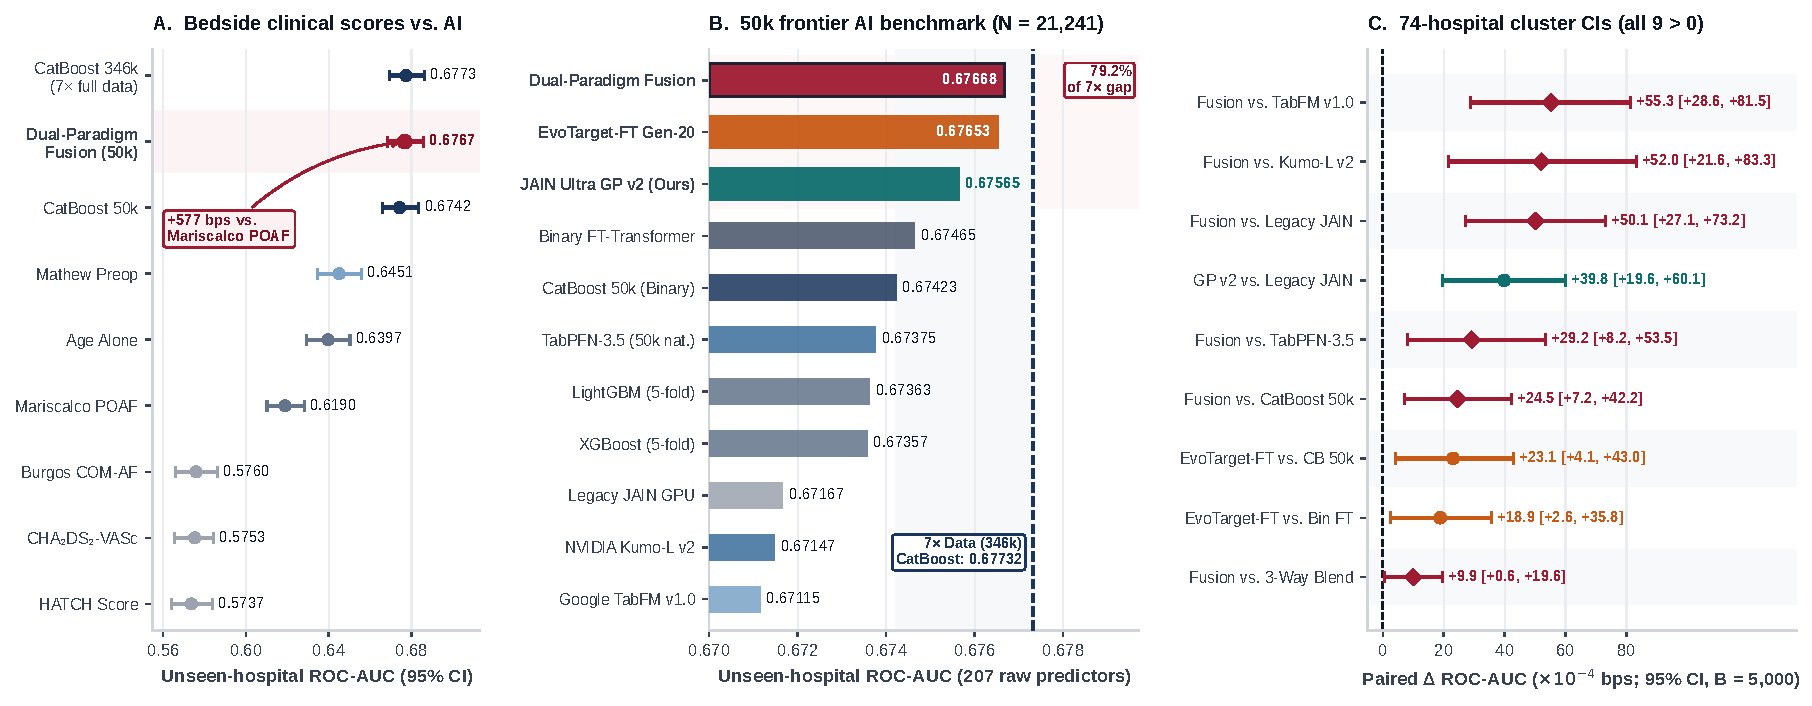
\includegraphics[width=\textwidth]{figures/fig2_primary_benchmark_and_forest.pdf}
  \caption{\ct{Primary Unseen-Hospital External Validation ($N=21{,}241$, 74 Unseen U.S.\ Hospitals, 207 Raw Pre-Incision Predictors).} \textbf{A},~Head-to-head ROC-AUC across six calibrated bedside clinical proxies, six world-leading 50k binary tabular model families, the proposed evolutionary and parallel-GP models, and the 7$\times$-larger 346k national full-registry CatBoost reference. \textbf{B},~Paired 5,000-draw 74-hospital cluster bootstrap contrasts ($\Delta$ ROC-AUC in basis points, $\times 10^{-4}$); filled diamonds indicate 95\% CIs strictly excluding zero. Dual-Paradigm Fusion outperforms every bedside proxy and every 50k binary baseline, including a 3-way binary neural--GBDT--TabPFN blend ($+9.9$ bps $[+0.6, +19.7]$).}
  \label{fig:primary_benchmark}
\end{figure*}

Both proposed paradigms broke above the 50k binary ceiling on identical 207 raw predictors: \textbf{JAIN Ultra GP v2} reached 0.6756 (95\% CI, 0.6673--0.6850), \textbf{EvoTarget-FT} (Gen-20 $z^*$) reached 0.6765 (0.6685--0.6856), and \textbf{Dual-Paradigm Fusion} achieved \textbf{0.6767 (0.6686--0.6858; AP~0.3777; ECE~0.0072; top-decile lift 1.84$\times$)}. Under 5,000-draw 74-hospital cluster bootstrapping (Table~\ref{tab:primary_results}; Figure~\ref{fig:primary_benchmark}B), Fusion decisively surpassed every bedside proxy---including $+577.0$ bps ($[+495.6, +656.9]$) over Mariscalco POAF and $+316.1$ bps over Mathew proxy---and outperformed every 50k binary AI baseline with 95\% cluster CIs strictly $>0$: $+55.3$ bps over TabFM, $+52.0$ bps over KumoTabular-Large, $+50.1$ bps over legacy JAIN GPU, $+31.1$ bps over XGBoost, $+30.5$ bps over LightGBM, $+29.2$ bps over TabPFN-3.5, $+24.5$ bps over CatBoost 50k, $+20.3$ bps over Binary FT, and $+9.9$ bps ($[+0.6, +19.7]$, $P>0=0.982$) over a 3-way binary blend (0.6757). Relative to 7$\times$-larger 346k CatBoost (0.6773), 50k Fusion recovered \textbf{79.2\%} of the scaling gap while surpassing 346k CatBoost in AP (0.3777 vs.\ 0.3776), ECE (0.0072 vs.\ 0.0076), 2017 unseen hospitals (0.6579 vs.\ 0.6578), and rare clinical tails (0.6935 vs.\ 0.6928), with identical performance excluding recorded preoperative AF ($n=21{,}103$; AUC~0.6771).

\subsection{1,000-Generation Target Evolution and Strictly Nested 2$\times$2 Causal Proof}
Tracking Stage-1 target evolution through 1,000 generations (256,000 fits; Figure~\ref{fig:target_evolution}A) confirmed rapid early denoising and asymptotic stability without collapse: EvoTarget-FT climbed from 0.67465 (Gen~0) to \textbf{0.67654} at Gen~20 ($+18.9$ bps $[+2.6, +35.8]$) and plateaued cleanly at 0.67592 through Gen~1,000 (CatBoost CE: $0.67408 \to 0.67538$ at Gen~20 $\to 0.67511$ at Gen~1,000). Replacing binary labels with Gen-20 continuous targets $z^*$ lifted unseen-hospital discrimination across \textbf{all seven independent architectures} (Figure~\ref{fig:target_evolution}B), with 5 of 7 cluster CIs strictly $>0$, including large gains on zero-shot tabular foundation model regressors: TabFM Reg $+97.2$ bps (beating binary TabFM Cls by $+26.7$ bps $[+3.7, +49.8]$), KumoTabular Reg $+27.9$ bps (beating binary Kumo Cls by $+35.2$ bps $[+9.0, +63.5]$), TabPFN-3.5 $5\times 10\text{k}$ Reg $+26.1$ bps, EvoTarget-FT $+18.9$ bps, and CatBoost $+12.9$ bps.

\begin{figure*}[t]
  \centering
  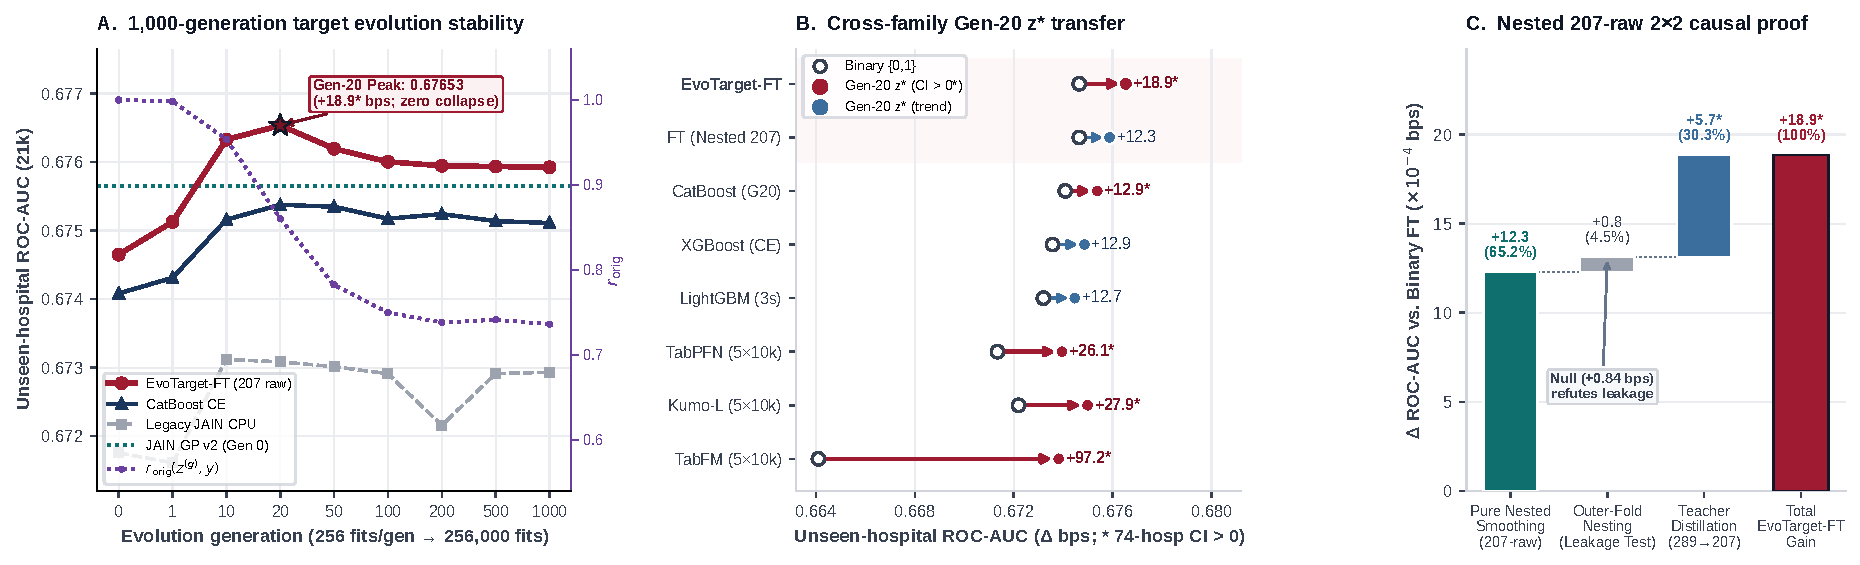
\includegraphics[width=\textwidth]{figures/fig3_target_evolution_and_causal_proof.pdf}
  \caption{\ct{1,000-Generation Target Evolution Stability, Cross-Architecture Transfer, and Strictly Nested 2$\times$2 Causal Audit.} \textbf{A},~External unseen-hospital ROC-AUC across nine milestones from Generation~0 to Generation~1,000 (256,000 cumulative Stage-1 fits), confirming peak discrimination at Gen~20 and a non-collapsing plateau through Gen~1,000. \textbf{B},~Replacing binary $\{0,1\}$ labels with Gen-20 continuous targets ($z^*$) yields positive unseen-hospital lift across all seven distinct tabular model architectures (three tabular foundation models, three GBDTs, and FT-Transformer), with five of seven paired 74-hospital CIs strictly exceeding zero. \textbf{C},~Exact 2$\times$2 causal decomposition separating genuine continuous-target denoising ($+12.3$ bps strictly nested on 207 raw predictors) from negligible outer-fold overlap ($+0.8$ bps, $P=0.68$) and Stage-1 teacher-feature distillation ($+5.7$ bps $[+0.3, +10.6]$).}
  \label{fig:target_evolution}
\end{figure*}

The strictly nested 2$\times$2 causal audit partitioned EvoTarget-FT's $+18.85$-bp gain into three exact mechanisms (Figure~\ref{fig:target_evolution}C): (1)~strictly nested 5-fold outer-loop 207-raw evolution (zero validation-hospital access) delivered \textbf{0.67588} ($+12.29$ bps $[-3.25, +28.53]$, $P>0=0.942$; 65\% of total gain); (2)~moving from nested to global 207-raw search added a statistically null $+0.84$ bps ($[-2.43, +4.40]$), ruling out outer-fold leakage; and (3)~Stage-1 privileged distillation of 82 clinical features into $z^*$ while keeping Stage-2 strictly on 207 raw predictors contributed a cluster-confirmed \textbf{$+5.72$ bps ($[+0.33, +10.61]$)}.

\subsection{JAIN Ultra GP v2 Engineering Rescue and Pre-Incision Physiological Drivers}
Resolving all six legacy JAIN bottlenecks drove a \textbf{$+39.8$-bp external rescue ($[+19.6, +60.1]$, $P>0=0.9998$)} from legacy GPU Gen-20 (0.6717) to the 6-family binary \textbf{JAIN Ultra GP v2} ensemble at \textbf{0.6756} (Figure~\ref{fig:gp_v2_interp}A), outperforming TabFM ($+45.0$ bps) and KumoTabular ($+41.8$ bps) standalone. Binary-$y$ early stopping rescued soft-target GP by $+9.1$ bps ($[+0.5, +18.0]$), while fresh-seed 7-fold hospital CV ($r=0.959$ on binary $y$) exposed $+55$-bp tree-to-tree OOF optimism on global $z^*$ explaining why binary-$y$ GP transported best (Figure~\ref{fig:gp_v2_interp}B). Even at Gen~0 (zero target evolution), blending JAIN Ultra GP v2 with Binary FT achieved 0.6762 with the lowest calibration error overall (ECE~0.0046; $+15.8$ bps $[+1.0, +30.3]$ over Binary FT).

\begin{figure*}[t]
  \centering
  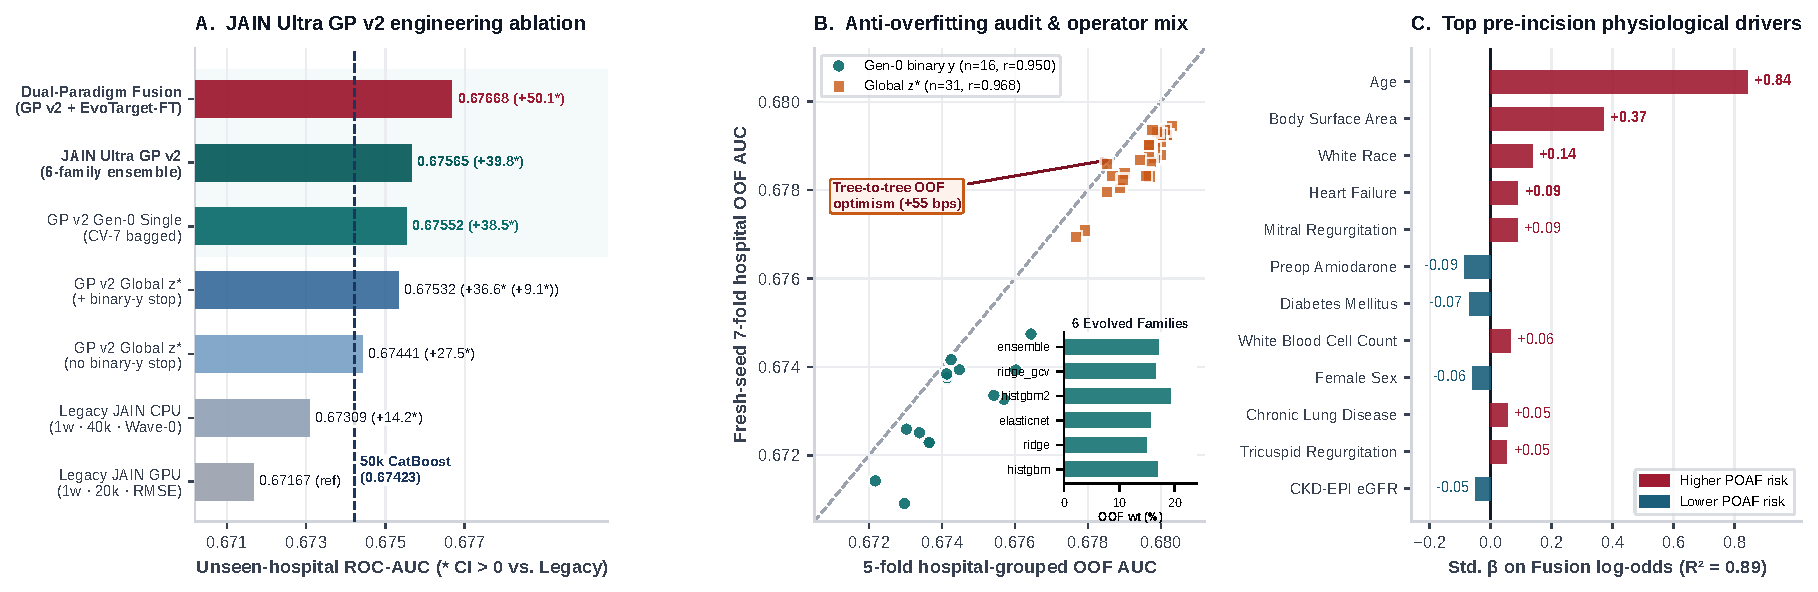
\includegraphics[width=\textwidth]{figures/fig4_jain_gp_v2_and_interpretability.pdf}
  \caption{\ct{JAIN Ultra GP v2 Engineering Rescue, Anti-Overfitting Verification, and Pre-Incision Physiological Drivers.} \textbf{A},~Stepwise external ROC-AUC rescue on 74 unseen hospitals from legacy JAIN GPU (0.6717) to JAIN Ultra GP v2 (0.6756, $+39.8$ bps $[+19.6, +60.1]$) and Dual-Paradigm Fusion (0.6767). \textbf{B},~Fresh-seed 7-fold vs.\ 5-fold hospital-grouped OOF verification across evolved Hall-of-Fame pipelines ($r=0.959$ on binary $y$), exposing $+55$-bp tree-to-tree OOF optimism on global $z^*$ and showing the balanced 6-family symbolic/linear/tree ensemble weights (inset). \textbf{C},~Top 12 standardized multivariable clinical drivers of Dual-Paradigm Fusion log-odds ($R^2 = 0.89$), showing concordant surgical pathophysiology including protective preoperative amiodarone ($\beta = -0.09$).}
  \label{fig:gp_v2_interp}
\end{figure*}

Log-odds from JAIN Ultra GP v2 and EvoTarget-FT correlated strongly yet imperfectly ($r=0.9591$), enabling orthogonal fusion. Standardized multivariable surrogate regression explained \textbf{89.0\%} ($R^2 = 0.8896$) of Dual-Paradigm Fusion log-odds variance with physiologically transparent pre-incision drivers (Figure~\ref{fig:gp_v2_interp}C): advancing age ($\beta=+0.84$), body surface area ($+0.37$), White race ($+0.14$), heart failure ($+0.09$), mitral regurgitation ($+0.09$), white blood cell count ($+0.06$), chronic lung disease ($+0.05$), and tricuspid regurgitation ($+0.05$) increased risk, whereas preoperative amiodarone ($\beta=-0.09$), diabetes ($-0.07$), female sex ($-0.06$), and preserved eGFR ($-0.05$) were independently protective.

\subsection{Calibration, Decile Stratification, and Decision Curve Clinical Utility}
Using development-only recalibration (zero test-label contact), Dual-Paradigm Fusion achieved near-ideal external calibration across 21,241 unseen-hospital cases (Figure~\ref{fig:calibration_dca}A): slope \textbf{0.983}, O:E \textbf{0.994}, 15-bin ECE \textbf{0.0072}, and ICI \textbf{0.0114}. Observed POAF rose monotonically across predicted deciles from \textbf{6.07\%} in D1 to \textbf{44.82\%} in D10---a \textbf{7.4-fold} risk separation with 1.84$\times$ top-decile enrichment (Figure~\ref{fig:calibration_dca}B).

\begin{figure*}[t]
  \centering
  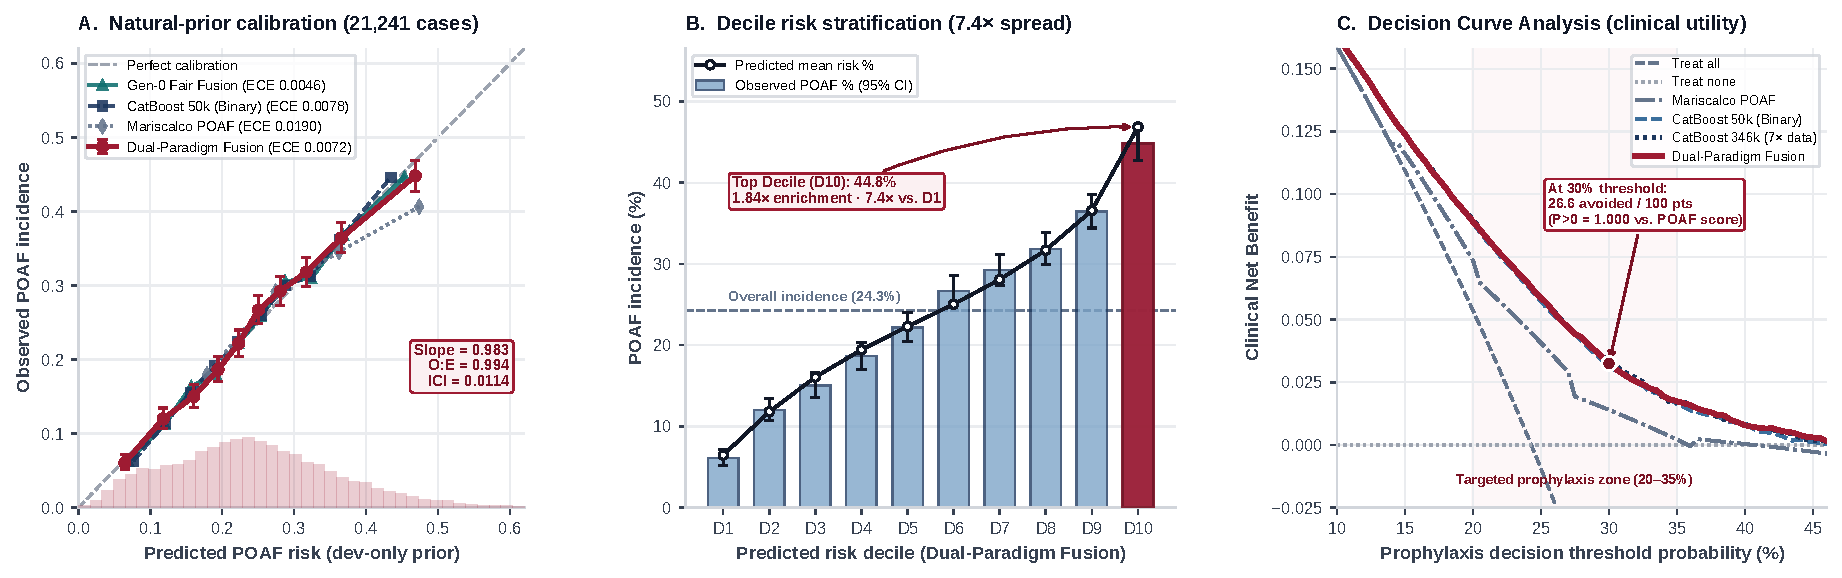
\includegraphics[width=\textwidth]{figures/fig5_calibration_stratification_dca.pdf}
  \caption{\ct{Clinical Calibration, Decile Risk Stratification, and Decision Curve Clinical Utility ($N=21{,}241$, 74 Unseen Hospitals).} \textbf{A},~Natural-prior calibration curves using strictly development-only recalibration (Bayes offset $-1.1365$), showing Dual-Paradigm Fusion alignment across deciles (slope~0.983, O:E~0.994, ECE~0.0072, ICI~0.0114). \textbf{B},~Monotonic risk stratification across predicted deciles from 6.07\% POAF in D1 to 44.82\% in D10 (7.4$\times$ gradient; 1.84$\times$ top-decile enrichment). \textbf{C},~Decision Curve Analysis demonstrating strictly superior Net Benefit across clinically actionable 15\%--40\% prophylaxis thresholds, avoiding 20.4--33.8 unnecessary interventions per 100 patients at 25\%--35\% thresholds ($P>0=1.000$ vs.\ Mariscalco POAF).}
  \label{fig:calibration_dca}
\end{figure*}

In Decision Curve Analysis (Figure~\ref{fig:calibration_dca}C; Supplementary Table~\ref{tab:supp_dca}), Fusion generated strictly positive Net Benefit across 15\%--40\% prophylaxis thresholds. At 25\%, 30\%, and 35\% decision thresholds (flagging 45.1\%, 29.3\%, and 17.5\% of patients), Fusion achieved Net Benefits of \textbf{0.0587}, \textbf{0.0325}, and \textbf{0.0174} (vs.\ negative values for universal prophylaxis), avoiding \textbf{20.4}, \textbf{26.6}, and \textbf{33.8 unnecessary prophylactic interventions per 100 CABG patients} and outperforming Mariscalco POAF across 100\% of hospital-cluster bootstrap draws ($P>0=1.000$).

\subsection{Demographic Equity and 74-Hospital Center Transportability}
Across 25 prespecified demographic, comorbidity, acuity, stress-slice, and hospital-volume strata (Figure~\ref{fig:equity_transport}A; Supplementary Table~\ref{tab:supp_subgroups}), Dual-Paradigm Fusion outperformed Mariscalco POAF in all 25 strata ($+374$ to $+1{,}333$ bps) and beat CatBoost 50k in \textbf{24 of 25 strata} (near-parity $-1.2$ bps in age $<60$~yr), maintaining strong performance across female (0.6891), male (0.6719), Black (0.6849), Hispanic/Latino (0.7146), diabetic (0.6812), LVEF $<40\%$ (0.6787), urgent/emergent (0.6830), rare-tail (0.6935), and low-, mid-, and high-volume center cohorts (0.6818--0.6851).

\begin{figure*}[t]
  \centering
  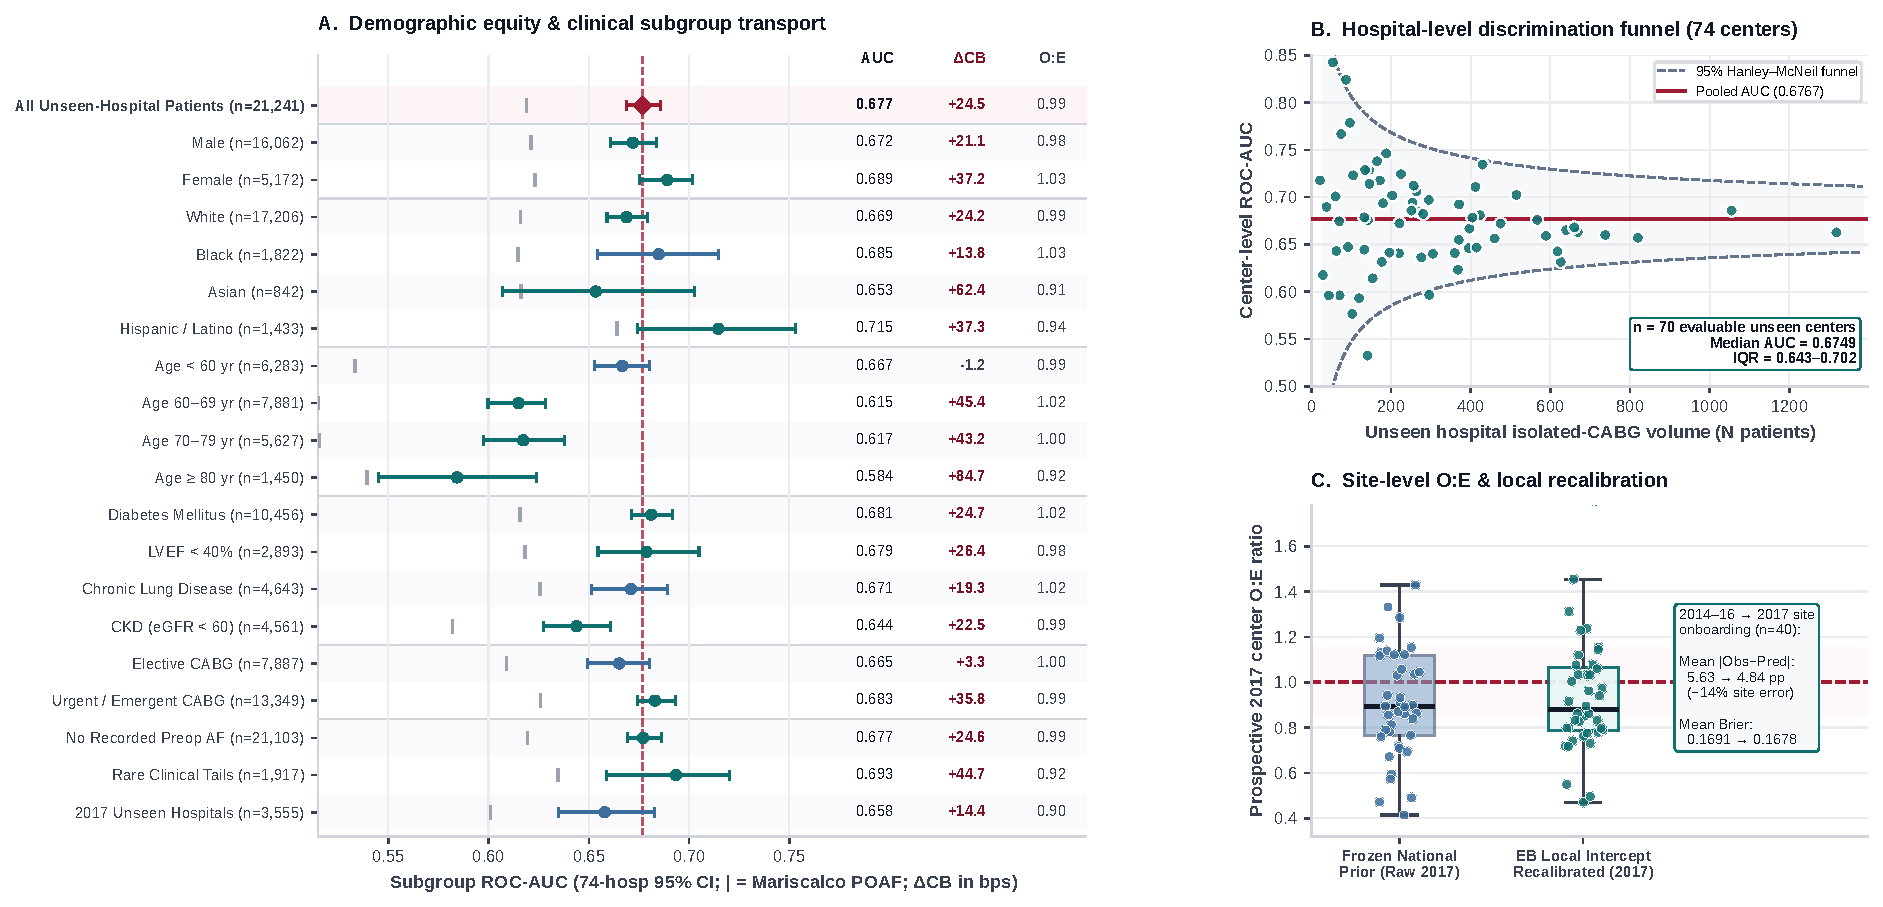
\includegraphics[width=\textwidth]{figures/fig6_equity_subgroups_and_hospital_transport.pdf}
  \caption{\ct{Subgroup Equity Audit, 74-Hospital Discrimination Funnel, and Prospective Local Intercept Recalibration.} \textbf{A},~Subgroup ROC-AUC (74-hospital 95\% CIs), $\Delta$ vs.\ CatBoost 50k (bps), and O:E ratio across demographic, comorbidity, acuity, and stress strata (vertical ticks show Mariscalco POAF). \textbf{B},~Hospital-level ROC-AUC across 70 evaluable unseen centers plotted against case volume within the 95\% Hanley--McNeil funnel (median AUC 0.6749, IQR 0.6434--0.7021). \textbf{C},~Prospective chronological site-onboarding recalibration (2014--2016 onboarding $\to$ 2017 deployment across 40 centers), showing that empirical-Bayes local intercept updating ($m_0=100$) lowers center-level mean absolute POAF rate error by 14\% (5.63 $\to$ 4.84~pp) and improves Brier score (0.1691 $\to$ 0.1678).}
  \label{fig:equity_transport}
\end{figure*}

Across 70 evaluable unseen hospitals, center-level AUCs tracked inside the 95\% Hanley--McNeil funnel (median \textbf{0.6749}, IQR 0.6434--0.7021; Figure~\ref{fig:equity_transport}B), while uncalibrated center O:E ratios reflected site incidence dispersion (median 0.958, IQR 0.856--1.135). In chronological prospective site onboarding (2014--2016 $\to$ 2017 across 40 centers; Figure~\ref{fig:equity_transport}C), updating a single empirical-Bayes local intercept ($m_0=100$) reduced prospective center mean absolute POAF rate error by \textbf{14\%} (5.63 $\to$ 4.84~pp) and improved Brier score (0.1691 $\to$ 0.1678).

\subsection{Seen-Hospital In-Network Deployment vs.\ Cold-Start Transport}
Evaluating every model on the matched \textbf{100.0\% Seen-Hospital} split (all 1,091 hospitals in training; 0 unseen test centers; $N=21{,}241$ holdout across 1,086 seen centers; Table~\ref{tab:seen_vs_unseen}; Figure~\ref{fig:seen_vs_unseen}) isolated hospital familiarity free of calendar confounding and yielded three clear findings.

\begin{table*}[t]
\centering\tablefont
\caption{\ct{Head-to-Head Transport Audit: Unseen-Hospital Cold Start (0\% Overlap, 74 Centers) vs.\ Seen-Hospital In-Network Deployment (100\% Overlap, All 1,091 Centers in Training; $N=21{,}241$ Natural-Prior Holdout).}}
\label{tab:seen_vs_unseen}
\setlength{\tabcolsep}{3.8pt}
\renewcommand{\arraystretch}{1.04}
\begin{tabularx}{\textwidth}{@{}Yrrrrrr@{}}
\toprule
\thd{Model Family} & \thd{Unseen Hosp.} & \thd{Seen Hosp.} & \thd{Seen + 50k} & \thd{Seen + 346k} & \thd{Site-Prior} & \thd{In-Net} \\
 & \thd{(0\% ovlp, 207)} & \thd{(100\%, 207 raw)} & \thd{EB Site Prior} & \thd{EB Site Prior} & \thd{Gain (bps)} & \thd{ECE} \\
\midrule
\multicolumn{7}{@{}l}{\textit{Bedside Clinical Proxy Reference}} \\
Mariscalco POAF Score (proxy) & 0.6190 & 0.6276 & --- & --- & --- & 0.0166 \\
\midrule
\multicolumn{7}{@{}l}{\textit{50,000-Patient Parity Benchmark (207 Raw Predictors $+$ Parameter-Free Closed-Form EB Hospital Priors)}} \\
Google TabFM v1.0.0 (5$\times$10k) & 0.6712 & 0.6775 & 0.6918 & 0.6986 & +210 & 0.0093 \\
NVIDIA KumoTabular-L v2 (5$\times$10k) & 0.6715 & 0.6764 & 0.6911 & 0.6977 & +213 & 0.0080 \\
XGBoost (5-fold binary) & 0.6736 & 0.6774 & 0.6895 & 0.6958 & +184 & 0.0100 \\
LightGBM (5-fold binary) & 0.6736 & 0.6780 & 0.6897 & 0.6960 & +180 & 0.0084 \\
PriorLabs TabPFN-3.5 (50k native) & 0.6738 & 0.6795 & 0.6919 & 0.6982 & +187 & 0.0086 \\
CatBoost 50k (5-fold binary) & 0.6742 & 0.6777 & 0.6902 & 0.6966 & +188 & 0.0089 \\
Binary FT-Transformer (Gen-0) & 0.6746 & 0.6784 & 0.6890 & 0.6958 & +174 & 0.0067 \\
JAIN Ultra GP v2 (6-family) & 0.6756 & 0.6788 & 0.6904 & 0.6969 & +181 & 0.0098 \\
EvoTarget-FT (Gen-20 $z^*$) & 0.6765 & 0.6793 & 0.6906 & 0.6972 & +179 & 0.0117 \\
\rowcolor{primarytint} \textbf{Dual-Paradigm Fusion (GP v2 $+$ FT)} & \textbf{0.6767} & \textbf{0.6794} & \textbf{0.6909} & \textbf{0.6974} & \textbf{+180} & \textbf{0.0110} \\
\midrule
\multicolumn{7}{@{}l}{\textit{50,000-Patient Native Site-Aware End-to-End Training (208 Features Including Train-Only 50k EB Prior)}} \\
CatBoost 50k (native \texttt{site208}) & --- & 0.6777 & 0.6886 & --- & +109 & 0.0117 \\
\rowcolor{primarytint} \textbf{Dual-Paradigm Fusion (native \texttt{site208}, \#1)} & \textbf{---} & \textbf{0.6794} & \textbf{0.6916} & \textbf{---} & \textbf{+121} & \textbf{0.0116} \\
\midrule
\multicolumn{7}{@{}l}{\textit{Full National Registry Reference ($7\times$ Larger Training Cohort, $N=346{,}454$, All 1,091 Centers)}} \\
CatBoost Full Registry (346k, 7$\times$) & 0.6773 & 0.6831 & --- & 0.7014 & +183 & 0.0083 \\
\bottomrule
\end{tabularx}
\par\smallskip\raggedright\fontsize{7.3}{9.1}\selectfont\color{sub}
In the Seen-Hospital split, all 1,091 U.S.\ centers appear in both the 346,454-case development set and the 50,000-case balanced benchmark (100.0\% overlap; 0 unseen test centers; exact matched $N=21{,}241$ holdout, 24.30\% POAF). Empirical-Bayes (EB) hospital priors are computed strictly from training rows with zero test-label contact. Among native 50k site-aware models, Dual-Paradigm Fusion (\texttt{site208}, 0.6916) strictly leads CatBoost \texttt{site208} ($+29.0$ bps $[+16.6, +41.5]$, $P>0=1.000$). Under closed-form $+\mathrm{EB}_{346\mathrm{k}}$ updating, all 50k models converge within 0.6958--0.6986 (cluster CIs overlapping zero); the slight additive edge of 10k-shard TFMs reflects $\sim$30\% lower implicit hospital entanglement ($r=0.088$--$0.092$ vs.\ $0.122$--$0.143$).
\end{table*}


\begin{figure*}[t]
  \centering
  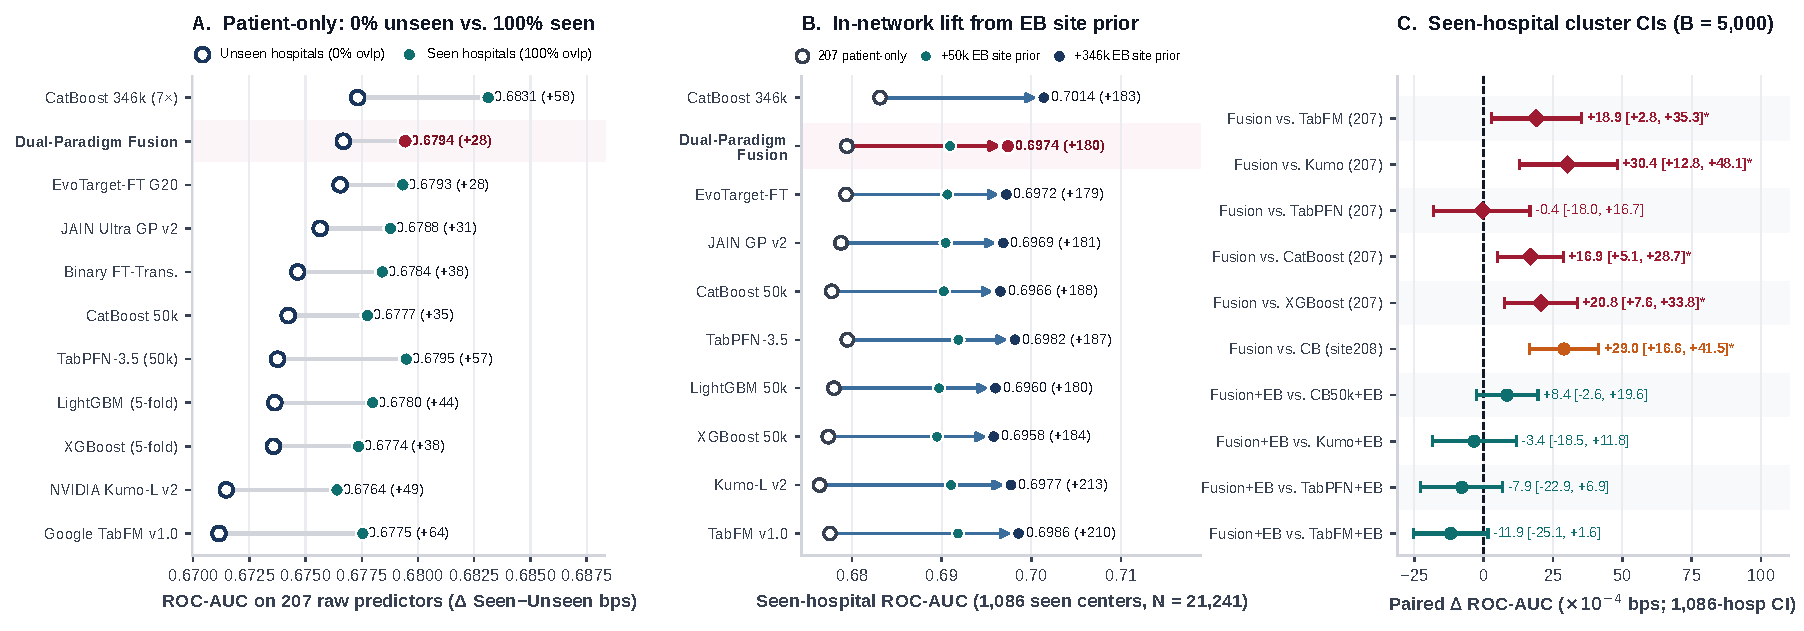
\includegraphics[width=\textwidth]{figures/fig7_seen_vs_unseen_hospitals.pdf}
  \caption{\ct{Unseen-Hospital Cold Start (0\% Overlap) vs.\ Seen-Hospital In-Network Deployment (100\% All-1,091-Hospitals-In-Train; $N=21{,}241$).} \textbf{A},~Patient-only discrimination on strictly 207 raw predictors (zero hospital identifiers): every algorithm gains $+28$--$64$ bps solely from hospital overlap, with tabular foundation models gaining roughly twice as much ($+49$--$64$ bps) as Dual-Paradigm Fusion ($+28$ bps). \textbf{B},~Adding strictly train-only empirical-Bayes hospital incidence priors vaults every 50k model by $+174$--$213$ bps into the 0.696--0.699 band and lifts 346k CatBoost to 0.7014. \textbf{C},~Paired 5,000-draw 1,086-hospital cluster bootstrap contrasts ($\Delta$ ROC-AUC in bps; asterisks denote 95\% CIs strictly excluding zero).}
  \label{fig:seen_vs_unseen}
\end{figure*}

First, even on strictly \textbf{207 patient-only predictors without hospital identifiers} (Figure~\ref{fig:seen_vs_unseen}A), hospital overlap inflated every algorithm by \textbf{$+28$ to $+64$ bps}. Tabular foundation models relied nearly twice as heavily on hospital familiarity---TabFM $+64$ bps ($0.6712 \to 0.6775$), TabPFN-3.5 native 50k $+57$ bps ($0.6738 \to 0.6795$), and KumoTabular $+49$ bps ($0.6715 \to 0.6764$)---as Dual-Paradigm Fusion ($+28$ bps, $0.6767 \to \mathbf{0.6794}$, Regime-1 locked weights) and JAIN Ultra GP v2 ($+31$ bps, 0.6788). Across 1,086 seen centers, patient-only Fusion strictly outperformed KumoTabular ($+30.4$ bps), XGBoost ($+20.8$ bps), TabFM ($+18.9$ bps), CatBoost 50k ($+16.9$ bps), LightGBM ($+14.5$ bps), and Mariscalco POAF ($+517.9$ bps; all CIs $>0$; Figure~\ref{fig:seen_vs_unseen}C), while tying TabPFN-3.5 native 50k ($-0.4$ bps $[-18.0, +16.7]$).

Second, incorporating each center's strictly train-only Empirical-Bayes (EB) historical incidence prior lifted every architecture by \textbf{$+174$ to $+213$ bps} (nearly $+2.0$ full AUC points; Figure~\ref{fig:seen_vs_unseen}B), boosting AP to 0.407--0.411, top-decile enrichment to 1.94--1.96$\times$, and 30\%-threshold Net Benefit to 0.042--0.044. Among native end-to-end 50k site-aware models (\cli{site208}), \textbf{Dual-Paradigm Fusion (\cli{site208})} ranked first at \textbf{0.6916 (0.6844--0.6987)}, beating CatBoost \cli{site208} (0.6887) by \textbf{$+29.0$ bps ($[+16.6, +41.5]$, $P>0=1.000$)}. Under closed-form Bayesian hospital-intercept updating with the 346k historical prior, all 50k models converged within \textbf{0.6958--0.6986} (Dual-Paradigm Fusion \textbf{0.6974}, $+179.6$ bps), while 346k Full-Registry CatBoost (\cli{site208}) crossed 0.70 at \textbf{0.7014 (0.6942--0.7087; AP~0.4109, ECE~0.0083, slope~1.014, O:E~0.999)}.

Third, correlating patient-only logits with true historical hospital POAF deviation ($\hat{\delta}_h^{\mathrm{EB}_{346\mathrm{k}}}$) uncovered \emph{implicit hospital fingerprinting}: models trained across 40k--346k patients from all 1,091 centers absorbed site-coding signatures without \cli{HospID} (CatBoost 346k $r=+0.1431$; Fusion $r=+0.1298$; CatBoost 50k $r=+0.1216$; TabPFN native 50k $r=+0.1184$), whereas 10k-context bagged foundation models (seeing $\sim$9 patients/center per shard) showed $\sim$30\% lower institutional entanglement ($r=+0.0878$--$0.0919$). Consequently, when combined additively with the explicit 346k hospital prior, 10k-shard TFMs avoided double-counting the site effect and edged slightly higher (0.6986 vs.\ 0.6974, cluster CIs spanning zero).
